\documentclass{article}
\usepackage{graphicx}
\usepackage[french]{babel}
\usepackage[T1]{fontenc}
\usepackage{hyperref}
\usepackage{algorithm2e}
\usepackage{tikz}
\usepackage[utf8]{inputenc}
\title{Rapport Projet : \\ Simulateur du jeu de la Vie}
\author{Quentin Levallois, Felix Bostock \\ L2 Informatique}
\date{\today}

\begin{document}

\maketitle

\includegraphics[scale=0.5]{logo.jpg}
\newpage
\tableofcontents
\newpage

\section{Introduction}
Dans le cadre, de nos études en 2ème années de licence Informatique, nous devions choisir un sujet pour la matière Conception Logicielle. Nous avons alors choisis le sujet du \textit{Jeu de la Vie} que l'on doit programmer en langage Java.
 Dans ce rapport nous allons commencer par vous faire une description de notre sujet et en expliquer les objectifs. Ensuite nous vous expliquerons l'architecture de notre projet ainsi que l'organistaion du travail. Après cela, on va expliquer comment implémenter l'algorithme de Hashlife et comment il peut être utiliser sur des exemples précis. Enfin nous ferons une rétrospéctive sur notre travail. 

\subsection{Description du générale du projet}
\textit{Le Jeu de la Vie} de John Conway, n'est pas un jeu au sens propre mais la simulation de l'évolution des cellules d'une grille autrement dit un automate cellulaire. Il se joue avec un joueur zero, ce qui veut dire qu'il n'a pas besoin de l'aide d'un utilisateur pour fonctionner.
\textit{Le Jeu de la Vie} se déroule sur une grille en 2 dimensions qui peuvent être petite ou infiniment grande. Chaque cellule de cette grille a un état qui peut être soit vivant soit mort. Une cellule a aussi 8 voisins qui sont tous adjacents que se soit verticalement, horizontalement ou diagonalement. 
Lors de chaque étape, on cherche à générer l'état suivant de chaque cellule grace à ses voisins grace au règles suivantes.
\begin{itemize}
    \item Règle 1 : Une cellule mort qui a trois voisins vivants devient une cellule vivantes.
    \item Règle 2 : Une cellule vivantes qui a 2 ou 3 voisins vivants reste une cellule vivantes.
    \item Règle 3 : Une cellule qui a soit 1 soit +3 voisins meurt et si elle est déjà morte elle ne change pas d'état.
\end{itemize}
Lorsque chaque étape est finit, on doit afficher l'update sur une interface. Cette interface devra afficher une grille qui devra l'update en temps par temps afin de pouvoir voir l'étape suivantes de chaque cellule de la grille. 

\subsection{Les objectifs du projet}

\textit{Le Jeu de la Vie} a des objectifs très clair, il doit pouvoir implémenter un automate cellulaire. Un automate cellulaire est une grille contenant des cellules qui elle même stocke des états(vivant ou mort) et qui peut évoluer en fonction du temps. Dans un deuxième temps, un autre objectif apparait. Elle consiste à créer une interface graphique permettant de visualiser \textit{le Jeu de la Vie}, elle permet aussi de pouvoir configurer une figure afin d'appliquer le programme sur cette dernière. L'interface devra aussi permettre à l'utilisateur de choisir un type de voisinage et un type de règle. Ensuite, notre \textit{Jeu de la Vie} devra implémenter l'algorithme de Hashlife. Ce dernier consiste à réduire au maximum les calculs afin de pouvoir appliquer notre \textit{Jeu de la Vie} sur des grilles de très grande taille.

\section{L'architecture du projet}
\subsection{L'arborescence des fichiers}
Pour notre projet on a décidé de clarifier notre dossier de la manière suivantte: 
\begin{itemize}
    \item Le premier dossier est le dossier build, il sert à stocker les fichiers compilés.
    \item le second dossier est le dossier src, il contient toutes les classes utilisés par le projets ainsi que tout le code.
    \item le dernier dossier est le dossier patterns, il contient tous les fichiers .txt contenant des patterns prédéfinies. 
\end{itemize}
\subsection{Les packages utilisés}
Pour respecter le principe du projet on a du faire adopté le Modèle Vue Controlleur(MVC) à notre projet.
C'est pour cela ,que l'on a décidé de dédier de packages différents pour chaque partie du code afin de pouvoir mieux le comprendre. Pour cela on peut voir que l'on a découper notre code en 3 packages, un pour l'interface nommé views, un pour les écouteurs du MVC que l'on a nommé listener ainsi que le dernier package nommé gameoflife qui contient tout les éléments lié au \textit{Jeu de la Vie}. 
\begin{itemize}
    \item Le package gameoflife : contient les éléments permettant de coder l'automate cellulaire ainsi que les quadtree utilisés pour utiliser l'algorithme de Hashlife. Ce package contient aussi le code lié au Hashlife.
    \item Le package listener : contient les éléments liés au écouteurs de l'interface.
    \item Le package views : contient les éléments liés à l'affichage de l'interface. Ce package contient toutes les classes permettant l'affichage de l'interface graphique du projet. Dont la grille du simulateur, les boutons \textbf{pause} et \textbf{play} ainsi que le bouton slider permettant de ralentir ou d'accélerer la vitesse d'affichage des nouvelles générations. 
\end{itemize}

\subsection{L'organisation du travail}
Le travail a été divisé en deux partie la première c'est le code de la grille, des classes quadtree et le hashlife qui a été fais à deux par Felix Bostock et Quentin Levallois. Et la deuxième partie Felix Bostock a fait la partie de l'interface graphique et Quentin Levallois a fait le rapport et le diaporama de la soutenance.


\section{Fonctionnalités implémentés}
\subsection{Le type de règle}
Le type de règle est important dans \textit{le Jeu de la Vie}. Il permet à l'automate cellulaire de se mettre à jour grace aux états suivants. Pour les règles, on a décidé de garder les règles de base car on a pas trouvé de règles convaincante à nos yeux.  

\subsection{Le type de voisinage}
Nous avons programmer la fonctionnalité \textbf{Type de Voisinage}. Cette dernière consiste à indiquer à notre grille comment son définie ses voisins. Dans le cas de base le voisinage est définie comme les 8 cellules autour de cette case. Nous avons fait en sorte que l'on puisse changer les règles de voisinage, on a pris pour exemples le fait de pouvoir dire que maintenant les voisins de notre cellules sont la case en haut, en bas, à gauche et à droite de la cellule. On peut donc dire que pour chaque cellule (x,y) ses voisins sont les cases (x+1,y) (x-1,y) (x,y+1) (x,y-1). Pour cela on a ajouté un bouton qui permet à l'utilisateur de pouvoir choisir entre le voisinage de base et le nouveau voisinage. Ce bouton appelle une fonction différente que le type de voisinage de base. Ainsi pour le nouveau voisinage, on prends la même grille que pour calculer le cas de base mais on change les cellules à sommer pour compter ce nouveau voisinage. 

\subsection{Le hashcode}
Comme dans chaque classe Java, on a du recodé le hashcode afin qu'il puisse 
être stocker sous un entier unique pour chaque noeud de l'arbre quadtree. Pour cela, on s'est dit que le meilleur moyen était de le programmer grace à sa valeur entière de la String du calcul de sa feuille comme vous pouvez le voir ci-dessous.

\begin{algorithm}
    \DontPrintSemicolon
    \KwIn{Node}
    \KwOut{l'entier de la String du calcul de la Node}
    \uIf{(this.level ==1)}{ \\
            int res\;
            res = this.cellNW == 1 ? 1000 : 0\; 
            res += this.cellNE == 1 ? 100 : 0\; 
            res += this.cellSW == 1? 10 : 0\; 
            res += this.cellSE == 1 ? 1 : 0\; 
            \Return {String.valueOf(res).hashCode()}\;
}       
        \Else{
        \Return (String.valueOf(this.nw.hashCode()) + 
                String.valueOf(this.ne.hashCode()) + 
                String.valueOf(this.sw.hashCode()) +
                String.valueOf(this.se.hashCode())).hashCode();
              }  
\caption {Algorithme du hashcode de nos noeud.}     
\end{algorithm}
Pour donner une explication claire de notre hashcode. Il consiste à aller au niveau 1 de chaque noeuds afin de sommer la valeur des 4 cellules de ce noeud. Après cela, il ferra le hashcode prédéfinie pour une string sur la string de la somme des 4 cellules. Si au contraire le niveau n'est pas égale à 1 alors il renverra le hashcode de la somme des 4 hashcode des noeuds( nw, ne, sw, se). Ce qui nous permet d'avoir pour chaque noeud donc pour chaque matrice un hashcode différent et plus ou moins unique. Je met plus ou moins unique, car il se peut qu'il y ait des cas ou le hashcode soit le même pour deux structures différentes donc nous le prendrons pas en compte. 

\subsection{La méthode equals}
La méthode equals doit elle aussi être redéfinis car elle est utile au hashlife afin de pouvoir réduire le nombre de calcul. Elle permet la vérification du hashcode dans notre table de hachage afin de savoir si elle a déjà été ajouter. Cette méthode est une comparaison entre de noeud afin de savoir si ces deux noeuds ont la même disposition.

\begin{algorithm}
    \DontPrintSemicolon
    \KwIn{deux noeuds}
    \KwOut{Vrai si les hashcode du noeud sont les même ainsi que que leurs niveau}
    \Return{this.hashCode() == a.hashCode() \textbf{et} \\ this.level == ((Node)a).getLevel(); }
\caption {Algorithme de la méthode equals de nos noeud.}     
\end{algorithm}

Pour savoir si un noeud equals un autre noeud il faut que les 2 noeuds ait les même hashcode ainsi que le même attribut level.



\subsection{L'algorithme du Hashlife}
L'algorithme du Hashlife est un algorithme consistant à traiter des cas complexes très rapidement. Pour cela, il utilise une table de hachage dans lequel il stocke des calculs déjà effectuer auparavant, afin de réduire au maximum le nombre de calcul ainsi que le temps de calcul.Cet algorithme se repose sur le fait de transformer notre matrice en quatre cellules où en quatre macrocellules de taille inférieur. Chacune des cellules a pour cela, un hashcode que l'on stockera dans une table de hachage. Cela réduira donc considérablement le nombre de calcul. 



\section{L'évolution du projet}
\subsection{Partie 1: les Matrice}
Pour commencer le projet, on a du faire le jeu de la vie sur une matrice.
On devait créer une matrice, la remplir aléatoirement et ensuite  calculer l'étape suivante grace au nombre de voisins pour chaque case. Le problème de cette version et qu'elle n'est pas du tout optimisé pour les grandes grilles.

\subsection{Partie 2: les Quadtree}
Ensuite, on a coder les matrices sous forme de quadtree. Cela nous a permis de voir comment on pouvez stocker correctement chaque matrice dans un quadtree afin de pouvoir faire les calculs sur un plus grands nombre de case. On peut faire le simulateur sur une matrice composé d'un grand nombre de cellules cependant, cette méthode ne nous permet pas assez de réduire les calculs. C'est pour cela qu'il a fallut qu'on fasse le Hashlife, ce dernier était censé stocker le hashcode de chaque noeud calculé dans une table de hachage afin que si le hashcode correspond à un hashcode déjà présent dans la table de hachage alors on reprend l'état suivant de ce noeud. Si ce n'est pas le cas alors on ajoute le hashcode dans la table de hachage. Ce dernier devrait nous faire réduire considérablement le nombre de calculs car nous n'avons pas besoin de faire es même calcul plusieurs fois notamment pour les grandes matrice qui peuvent être vide sur 3/4 . Cette algorithme devrait nous permetre d'identifier que ce coté de la matrice est vide est donc qu'il ne sert à rien de calculer les cellules vides. On aura juste à remplacer la partie vide de la matrice par la même partie vide. Par exemples :

 



\section{Quelques exemples de Jeu de la vie fait par fichier .txt}
Quelques exemples codés par fichier .txt on pu être réaliser notamment, celui du triangle, on peut voir que le shéma de base est un triangle et que celui d'arriver est un duo, ce qui veut dire que lorsque le programme va à l'état suivant. A la fin de ces états suivants, ils restent alors que deux matrices l'une qui fait un trait horizontal au centre du triangle du début et une autre avec un trait vertical qui lui aussi sera au centre du triangle de base.
Pour cela, il a fallu que l'on fasse un interpreteur de matrice qui prends un fichier .txt en entrée et qui le lit afin de le transformer en matrice. Lorsque cette matrice est créer on peut alors utiliser notre programme principale du jeu de la vie sur cette matrice.  
Afin de pouvoir utiliser chacune des figures on a programmer un menu déroulant permettant à l'utilisateur de changer le fichier .txt.

\section{L'interface Graphique}
Notre Interface graphique doit respecter le MVC autrement dit le Modèle Vue Controlleur.
Au lancement du programme principal, une fenêtre apparait. Cette fenêtre contient plusieurs éléments notamment une barre afin de choisir une figure parmis les figures déjà préécris. Elle a aussi, une grille permettant de voir graphiquement le jeu de la vie sur l'exemple choisis ou alors elle peut aussi, vous permettre de vous même dessiner une figure. Cette interface a deux bouton, un bouton play vous permettant de lancer le programme sur la figure choisis et un bouton pause vous permettant de stopper momentanement le programme à un moment choisis. Il y a aussi un bouton slider qui vous permet d'accélérer ou de ralentir l'affichage des nouvelles générations de votre figure. L'interface a aussi un mode pour choisir quelle règles le type de voisinage. L'utilisateur a deux choix de voisinage, soit celui de base soit celui expliquer au dessus.

\begin{figure}[!ht]
    \centering
    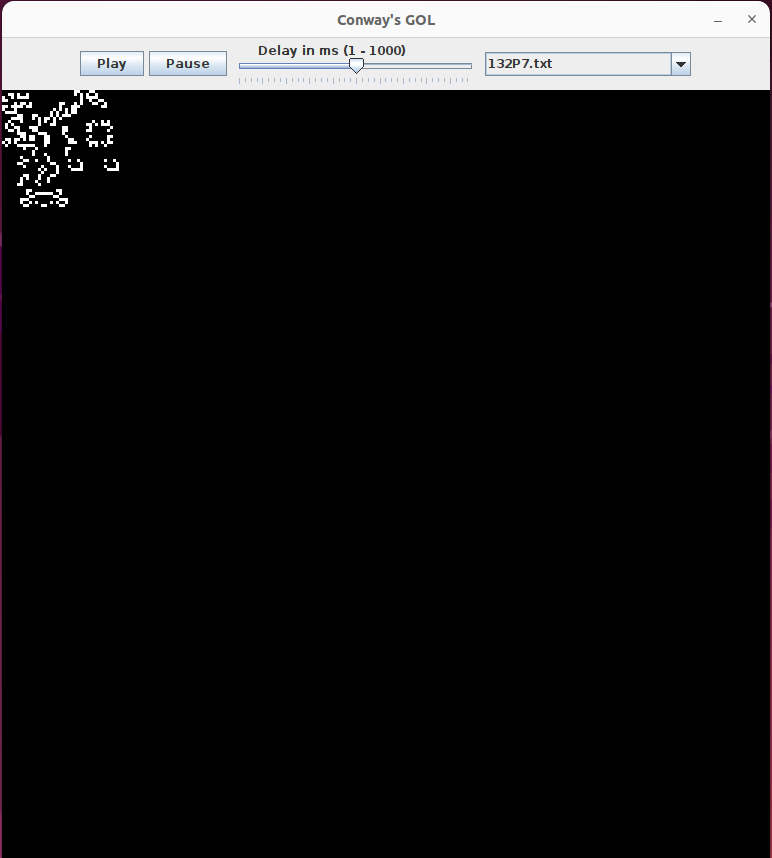
\includegraphics[scale=0.5]{interface.png}
    \caption{Interface du Jeu de la Vie}
\end{figure}

\newpage
\section{Conclusion}
Le rendu final vous propose un simulateur du jeu de la vie fonctionnel utilisant l'algorithme du Hashlife. L'interface respecte le Modele Vue Controlleur. Elle vous propose de tester l'algorithme sur des fichier .txt déjà préécris comme le triangle où d'autres exemples ainsi que le fait de pouvoir vous même cliquer sur la matrice afin de faire vos propre figures et leurs appliquer le jeu de la vie.
\end{document}
